\begin{center}
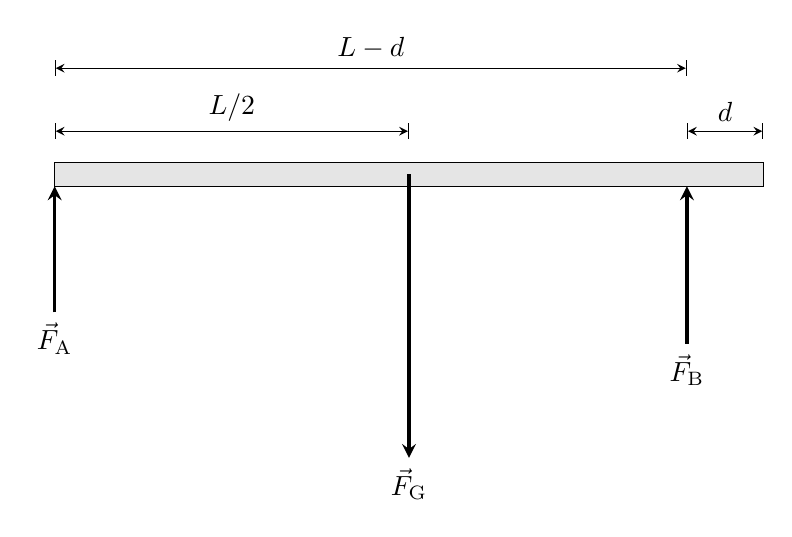
\begin{tikzpicture}[>=stealth]
 \fill[gray!20] (0,0) rectangle (9,0.3);
 \draw (0,0) rectangle (9,0.3);
 \draw[->, very thick] (0,-1.6) -- (0,0) node[pos=0, below] {$\vec F_\mathrm{A}$};
 \draw[->, very thick] (8.03,-2.0) -- (8.03,0) node[pos=0, below] {$\vec F_\mathrm{B}$};
 \draw[->, very thick] (4.5,0.15) -- (4.5,-3.45) node[below] {$\vec F_\mathrm{G}$};
 \draw[|<->|] (0,0.7) -- (4.5,0.7) node[midway, above] {$L/2$};
 \draw[|<->|] (0,1.5) -- (8.03,1.5) node[midway, above] {$L-d$};
 \draw[|<->|] (8.03,0.7) -- (9,0.7) node[midway, above] {$d$};
\end{tikzpicture}
\end{center}

Die Gewichtskraft $F_\mathrm{G}$ des Balkens greift in seiner Mitte an. Arbeiter A stützt am Ende, Arbeiter B im Abstand $L-d$ davon. Wir wählen den Auflagepunkt von A als Drehachse; das Drehmoment von $F_\mathrm{A}$ ist dann null:
\begin{align}
 F_\mathrm{B}\cdot\left(L-d\right) &= F_\mathrm{G}\cdot\frac{L}{2} \\
 \frac{F_\mathrm{B}}{F_\mathrm{G}} &= \pBaF = \frac{\LBa}{2\cdot\left(\LBa-\dBa\right)} = \pBa \approx \result{\pBaP{0}{2}}
\end{align}
Wegen $F_\mathrm{A} + F_\mathrm{B} = F_\mathrm{G}$ trägt A den Rest:
\begin{align}
 \frac{F_\mathrm{A}}{F_\mathrm{G}} &= \pAaF = \pAa \approx \result{\pAaP{0}{2}}
\end{align}
Der Arbeiter näher bei der Mitte trägt mehr als die Hälfte.
